\documentclass[twocolumn]{article}
\usepackage[utf8]{inputenc}
\usepackage{biblatex}
\usepackage{listings}
\usepackage{graphicx}
\graphicspath{ {./images/} }
\addbibresource{bibliography.bib}


\title{Compiler Annotation Solutions for Concurrent Information Flow Security}
\author{Alexander Blyth}
\date{August 2020}

\begin{document}
\maketitle

% TODO: Fix refs of security policy of vars vs. data


\textbf{\textit{Abstract} - Information flow security in concurrency is difficult due to the increasing complexity introduced with multiple threads. Additionally, compiler optimisations can break security guarantees that have been verified in source code. In this paper, we propose a thesis to explore these issues through providing annotations in C source code that propagate through to the binary or assembly. These annotations could then be used to guide a static analysis of information flow security in concurrency. This approach involves (1) capturing C source code annotations provided by the user about the security policy of data and variables and (2) passing these annotations down to the binary where static analysis tools can be utilised to identify security vulnerabilities in the produced binary. }

\section{Topic Definition}
TODO: Brief overview of the background of the topic

- provide a tool to analyse C programs to detect security violations created through information flow control through wpif.

- Analysis done after compilation to a binary to detect information flow violations introduced by compiler optimisations

- Explore ways to preserve annotations in C through compilation to binary with minimal modification to the compiler

\section{Background}
Vulnerabilities in software can lead to catastrophic consequences when manipulated by attackers. \textit{Example in here?}
% Maybe talk about heartbleed?

\subsection{Information Security}

Computer security is defined as a preservation of \textbf{integrity}, \textbf{availability} and \textbf{confidentiality} of information, and extends to include not only software but hardware, firmware, information, data and telecommunications \cite{guttman1995introduction}.
Confidentiality requires that data is not available to unauthorised users, and that individuals can control what information can be collected and disclosed to others. Data integrity requires that only authorised sources can modify data, and that the system can perform tasks without interference from outside sources. Finally, availability of a system requires that service is not denied to authorised users. Together, these principles create the CIA triad \cite{stallings2012computer}. To enforce a secure system, all three principles must be upheld.

Modern programs are becoming increasingly complex with potential for networking, multi-threading and storage permissions and more. As such, security mechanisms must be put in place to verify and enforce the information security requirements. The adequacy of a security mechanism depends on the adversary model. The adversary model is a formal definition of the attacker and their abilities in a system, and defines who we are protecting against \cite{do2019role}. Ideally we would like to design a system to protect against the strongest adversary or attacker, however, this is often not required or even possible. Instead, we must consider the security policy, security mechanism and strongest adversary model to make a system secure \cite{balliu2014logics}.

Standard security processes that handle access control such as a firewall or antivirus software can fail as they do not constrain where information is allowed to flow, meaning that once access is granted it can propagate to insecure processes where it can be accessed by attackers. Where a large system is being used, it is often the case that not all components of the codebase can be trusted, often containing potentially malicious code \cite{sabelfeld2003language}. Take for example your modern-day web project. Where a package manager such as Node Package Manager (npm) could be used to utilise open-source packages to speed up development progress, it could also inadvertently introduce security vulnerabilities. Rewriting all packages used to ensure security would be time-consuming and expensive and is not a viable option. Instead, controlling where information can flow and preventing secure data from flowing into untrusted sources or packages can maintain confidentiality of a system.

One may suggest runtime monitoring the flow of data to prevent leakage of secure data. Aside from the obvious computational and memory overhead, this method can have its own issues. Although it can detect an \textit{explicit} flow of data from a secure variable to a public variable, it is unable to detect \textit{implicit} data flow, where the state of secure data can be inferred from the state of public data or a public variable \cite{denning1977certification}. Take for example figure \ref{fig:implicit}. In this example, a public, readable variable is initially set to the value of 1. There is also a secret variable which may contain a key, password or some other secret that must be kept secure from any attackers. Depending on the value of the secret variable an attacker can infer information about this variable depending on whether the value of the public variable is updated to a value of 0. Assuming that the inner workings of the system is known by the attacker, information about the secret variable can be leaked \textit{implicitly} and inferred by the state of public variables.

\begin{figure}
    \begin{lstlisting}
secret := 0xC0DE mod 2
public := 1
if secret = 1
    public := 0
        \end{lstlisting}
    \caption{Implicit flow of data to a public variable}
    \label{fig:implicit}
\end{figure}

Security concerns do not only exist at the application level. In a huge codebase such as an OS, different low-level bugs can be exploited to gain access to data, such as by using buffer overflows to inject viruses or trojans \cite{agten2012recent}. However, most security failures are due to security violations introduced at the application level \cite{jang2010empirical}. Therefore, this thesis will focus primarily on security concerns at the high level.

\subsection{Information Flow Control}
As seen by the issues that can be introduced via implicit and explicit flow of data, there is room to improve on the existing techniques imposed by current security measures. To protect confidentiality, secure or sensitive information must be prevented from flowing into public on insecure variables. Additionally, to protect integrity, untrusted data from public sources must be prevented from flowing into secure or trusted destinations \textit{From my understanding, we don't care about this in this thesis?} \cite{balliu2014logics}. An information flow security policy can be introduced to classify or label data, or more formally, a set of \textit{security levels} to which each object is bound by across a multi-level security lattice \cite{denning1976lattice}.

Many security levels can be identified to classify different classes of objects, however, for now we will consider two security levels: high and low. Data labelled as high signifies that the data is secret, and low data is classified as non-sensitive data, such that it does not need to be protected from an attacker or adversary. Variables that can hold data in a program can additionally be classified as high or low as a \textit{security classification}. A variable's security classification shows the highest classification of data it can safely contain \cite{winter2020information}. A high variable can hold both high and low data, whereas a low variable which is visible to an attacker can only safely hold low data. As mentioned previously, confidentiality must be upheld by preventing high or secret data from flowing to low or public variables where an attacker can observe it. The permitted flow of data can be observed in \ref{fig:flow}. Note that high data is not allowed to flow into low variables.

\begin{figure}
    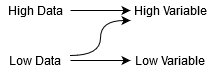
\includegraphics{flow.png}
    \caption{Permitted flow of data}
    \label{fig:flow}
\end{figure}

\subsection{Information Flow Security in Concurrency}
Controlling the flow of information is a difficult problem, however, this is only exacerbated in concurrent programs, which are a well known source of security issues \cite{mantel2014noninterference}\cite{smith2019value}\cite{vaughan2012secure}. Research has been conducted into concurrent programs to explore ways the security of concurrent programs can be verified. Mantel et al. \cite{mantel2011assumptions} introduced the concept of assumption and guarantee conditions, where assumptions are made about how concurrent threads access shared memory and guarantees are made about how an individual thread access shared memory that other threads may rely upon. Each thread can be observed individually using assumptions that can be then used to prove a guarantee about that individual thread. This concept of assumptions (or rely) and guarantee conditions can reduce the complexity of dealing with concurrency in threads and assist in verifying the correctness of information flow security in concurrency. However, this approach is limited in the types of assumptions and guarantees it supports. Building on this, Murray et al. \cite{ernst2019seccsl} \cite{murray2018covern} provide information flow logic on how to handle dynamic, value-dependent security levels in concurrent programs. In this case, the security level of a particular variable may depend on one or more other variables in the program. As such, the variable's security level can change as the state of the program changes. This logic is essential where the security level of data depends on its source. However, this approach is not sufficient when analysing non-blocking programs. The approach relies heavily on locks which block particular threads from executing. This in turn leads to slower processing due to blocked threads \cite{prakash1991non}.

To overcome information flow security in non-blocking concurrent threads, Winter et al. \cite{winter2020information} explores verifying security properties such as non-interference through the use of general rely/guarantee conditions using backwards, weakest precondition reasoning. Ideally a tool could be created to verify security policies required for sensitive processes. Users of this system could provide rely/guarantee conditions for each thread as well as security levels for data and variables i.e. high or low data and variables. Working backwards through the execution of the program, violations of the security policy will be detected. Detected violations could be due to an incorrect assumption of the rely and guarantee conditions or a failure to uphold the security policy. This thesis will focus on the compilation stage of this tool.
% TODO: Talk more about wpif, not sure what exactly to discuss about it here? - implicit & explicit, - user defined rely/guarantee conditions - uses of a tool?
% Is it a static analysis of the binary of a compiled program?
% I'd like to include a diagram here to show how the tool would be used

\subsection{Compilers and Security}
Compilers are well known to be a weak link between source code and the hardware executing it. Source code that has been verified to provide a security guarantee, potentially using formal techniques, may not hold those security guarantees when being executed. This is caused by compiler optimisations that may be technically correct, however, subvert the expectations a programmer may have about the execution of their program \cite{d2015correctness}. This problem is known as the \textit{correctness security gap}. One example of the correctness security gap is caused by an optimisation called dead store elimination. Figure \ref{fig:deadstore} was derived from CWE-14 \cite{cwe14} and CWE-733 \cite{cwe733} and used by D'Silva et al. \cite{d2015correctness}. Here a secret key was retrieved and stored in a local variable to perform some work. After completing the work, and to prevent sensitive data from flowing into untrusted sources, the key is wiped from memory by assigning it the value 0x0.

\begin{figure}
    \begin{lstlisting}
crypt() {
    key := 0xC0DE // Read key
    ... // Work with the key
    key := 0x0 // Clear memory
}
        \end{lstlisting}
    \caption{Implicit flow of data to a public variable \cite{d2015correctness}}
    \label{fig:deadstore}
\end{figure}

From the perspective of the source code, a programmer would expect the sensitive data from key to be scrubbed after exiting the function. However, key is a variable local to the function. As key is not read after exiting the function, the statement that assigns key to a value of 0x0 will be removed as part of dead store elimination. This results in lingering memory that could be exploited by an attacker. In GCC, with compiler optimisations on, dead store elimination is performed by default \cite{gccoptimise}. Additionally, dead store elimination has been proven to be functionally correct \cite{benton2004simple}\cite{leroy2006formal}.

% TODO: Discuss what other compiler optimisations can cause the correctness security gap

This leads to the question, \textit{what security guarantees in source code are being violated by compiler optimisations?} Although one could analyse each individual compiler optimisation to check for potential security violations in source code, defensively programming against the compiler can be counter-initiative. One might also suggest turning compiler optimisations off, however, this leads to slower code. In a concurrent system where execution time is critical, turning compiler optimisations off is not a viable option. Instead an alternative solution is to perform a static analysis on binary or assembly for security violations. As compilation has already been executed, such analysis would reveal security guarantee violations that result due to compiler optimisations.

\subsection{Compilation Annotations}
This project can take two routes; the proposed tool will be required to run an analysis on either binary or assembly. For either route, annotations used to guide a static security analysis will need to be provided by the user in the C programs they write. The tool will then be required to propagate these annotations down to compiled forms, i.e. binary or assembly. From here, a static analysis can be conducted as described by Winter et al. \cite{winter2020information}. Ideally these annotations can be propagated through with little to no modification of the C Compiler being used as to reduce complexity and increase modularity and reusability of such a a tool. However, it is unclear as to whether passing annotations down with no modification to the compiler is currently possible. In this thesis, this issue will be explored. 

Running a static analysis on a binary can be difficult due to the low level nature of a binary file. As such, to sufficiently perform such an analysis, the binary would be required to be decompiled to a higher-level form, such as an assembly file. From here a static analysis could be conducted. The alternative approach would be to perform the analysis directly on the compiled assembly output files rather than reducing these to binary. Currently, it is unclear as to what compiler optimisations are made when reducing an assembly file to binary, and will be explored further throughout the lifetime of this thesis. In GCC, "temporary" intermediate files can be stored using the flag \textit{save-temps} \cite{gccdevoptions}. These stored files can then be used for analysis. 

% TODO: Include figure of this problem

% TODO: Symbol table.

\subsection{Similar Solutions}
In safety-critical real-time software such as flight control systems, it is required to analyse the \textit{Worst Case Execution Time} (WCET). This kind of analysis can be conducted using static analysis tools to estimate safe upper bounds. In the case of AbsInt's aiT tool this analysis is conducted alongside compiler annotations to assist where loop bounds cannot be computed statically. In these cases, the user can provide annotations to guide the analysis tools \cite{schommer2018embedded}. This tool builds on an existing annotation mechanism that exist in CompCert, a C compiler that has been formally verified for use in life-critical and mission-critical software \cite{compcert}\cite{leroy2016compcert}. CompCert annotations are not limited to WCET analysis. A general mechanism for attaching free-form annotations that propagate through to assembly files can be achieved with CompCert. This approach is able to reliably transmit compiler annotations through to binary through method calls which are carried through compilation and the linked executable without using external annotation files. CompCert prints annotation strings as a comment in the generated assembly code, and an additional tool is used to parse these comments and generate annotations. However, due to its treatment as an external function, annotations cannot be placed at the top level of a compilation unit, unlike a variable declaration. 

% Fix: Additionally, care needs to be taken to avoid compiler optimisations removing annotations or rendering annotations inapplicable after optimisation.

A similar approach to CompCert is used by The ENTRA (Whole-Systems ENergy TRAnsparency). As part of providing a common assertion language, pragmas are used to propagate information through to comments in the assembler files. Information is retained in LLVM IR and ISA representations. However, these annotations are not stored in the final binary and thus comments must be extracted from assembler files \cite{eder2013common}.

TODO: Discuss Vu et al. approach to compiler annotations through LLVM. 
ACSL
% Vu et al. \cite{vu2020secure} explore creating a static analysis tool for analysing code for ... using LLVM that preserve properties through compiler optimisations. 

% Li et al. 
% - Li, Puat and Rohou present framework where source code annotations are transformed into annotations on the binary level
% - Focus on loop count annotations and preservation through classic loop optimisations

% GCC plugins: https://gcc.gnu.org/wiki/plugins

\section{Project Plan}

Milestones:
\begin{itemize}
    \item Investigation into C Compiler annotation solutions and approaches
    \begin{itemize}
        \item Thesis Proposal
        \item Literature Review
        \item Source Code inspection of AbsInt's, ENTRA and Vu et al. tools
        \item Workspace set up
    \end{itemize}
    \item Tool development
    \item Testing \& Correctness evaluation of tool
    \item Benchmarking and Performance Testing
\end{itemize}

\section{Risk Assessment}
This project will be conducted primarily using a home workstation. Risk low.
% - WPIF

% - Language-based security
%     - Java language-based security
%     - Annotations as a solution

% - Avoid modifying Compiler
%     - reduce complexity
%     - avoid updating tool for each compiler update
%     - potential for reusability for other languages / compilers

% - Mandatory Access control See: Language-Based Information-Flow Security Andrei Sabelfeld and Andrew C. Myers

\printbibliography

\end{document}

